% THIS DOCUMENT IS FOLLOWS THE VOLERE TEMPLATE BY Suzanne Robertson and James Robertson
% ONLY THE SECTION HEADINGS ARE PROVIDED
%
% Initial draft from https://github.com/Dieblich/volere
%
% Risks are removed because they are covered by the Hazard Analysis
\documentclass[12pt]{article}

\usepackage{booktabs}
\usepackage{tabularx}
\usepackage{graphicx}
\usepackage{hyperref}
\usepackage{enumitem}
\usepackage{longtable}
\hypersetup{
    bookmarks=true,         % show bookmarks bar?
      colorlinks=true,      % false: boxed links; true: colored links
    linkcolor=red,          % color of internal links (change box color with linkbordercolor)
    citecolor=green,        % color of links to bibliography
    filecolor=magenta,      % color of file links
    urlcolor=cyan           % color of external links
}

\newcommand{\lips}{\textit{Insert your content here.}}
\newcounter{reqnum} %Functional requirement number
\newcommand{\rthereqnum}{FR\refstepcounter{reqnum}\thereqnum:}
\newcommand{\frref}[1]{FR\ref{#1}}

\newcounter{uhrnum} %Usability and Humanity Requirement number
\newcommand{\rtheuhrnum}{UHR\refstepcounter{uhrnum}\theuhrnum:}
\newcommand{\uhrref}[1]{UHR\ref{#1}}

\newcounter{oernum} %Operational and Environmental Requirement number
\newcommand{\rtheoernum}{OER\refstepcounter{oernum}\theoernum:}
\newcommand{\oerref}[1]{OER\ref{#1}}

\newcounter{srnum} %Security Requirement number
\newcommand{\rthesrnum}{SR\refstepcounter{srnum}\thesrnum:}
\newcommand{\srref}[1]{SR\ref{#1}}

\newcounter{cprnum} %Compliance  Requirement number
\newcommand{\rthecprnum}{CPR\refstepcounter{cprnum}\thecprnum:}
\newcommand{\cprref}[1]{CR\ref{#1}}

%% Comments

\usepackage{color}

\newif\ifcomments\commentstrue %displays comments
%\newif\ifcomments\commentsfalse %so that comments do not display

\ifcomments
\newcommand{\authornote}[3]{\textcolor{#1}{[#3 ---#2]}}
\newcommand{\todo}[1]{\textcolor{red}{[TODO: #1]}}
\else
\newcommand{\authornote}[3]{}
\newcommand{\todo}[1]{}
\fi

\newcommand{\wss}[1]{\authornote{blue}{SS}{#1}} 
\newcommand{\plt}[1]{\authornote{magenta}{TPLT}{#1}} %For explanation of the template
\newcommand{\an}[1]{\authornote{cyan}{Author}{#1}}

%% Common Parts

\newcommand{\progname}{Course Buddy} % PUT YOUR PROGRAM NAME HERE
\newcommand{\authname}{Team \#5, Overwatch League
\\ Jingyao, Qin
\\ Qianni, Wang
\\ Qiang, Gao
\\ Chenwei, Song
\\ Shuting, Shi
\\ } % AUTHOR NAMES                  

\usepackage{hyperref}
    \hypersetup{colorlinks=true, linkcolor=blue, citecolor=blue, filecolor=blue,
                urlcolor=blue, unicode=false}
    \urlstyle{same}
                                

\newcounter{udreqnum} %User documentation requirement number
\newcommand{\rtheudreqnum}{UDR\refstepcounter{udreqnum}\theudreqnum:}
\newcommand{\udrrref}[1]{UDR\ref{#1}}
\newcounter{utreqnum} %User training requirement number
\newcommand{\rtheutreqnum}{UTR\refstepcounter{utreqnum}\theutreqnum:}
\newcommand{\utrref}[1]{UTR\ref{#1}}



\newcounter{mreqnum} %Maintenance Requirements number
\newcommand{\rthemreqnum}{MR\refstepcounter{mreqnum}\themreqnum:}
\newcommand{\mrrref}[1]{MR\ref{#1}}


\newcounter{sreqnum} %Supportability Requirements number
\newcommand{\rthesreqnum}{SR\refstepcounter{sreqnum}\thesreqnum:}
\newcommand{\srrref}[1]{SR\ref{#1}}

\newcounter{areqnum} %Adaptability Requirements number
\newcommand{\rtheareqnum}{AR\refstepcounter{areqnum}\theareqnum:}
\newcommand{\arrref}[1]{AR\ref{#1}}

\newcounter{creqnum} %Cultural Requirements number
\newcommand{\rthecreqnum}{CR\refstepcounter{creqnum}\thecreqnum:}
\newcommand{\crrref}[1]{CR\ref{#1}}


\begin{document}

\title{Software Requirements Specification for \progname} 
\author{\authname}
\date{\today}
	
\maketitle
~\newpage

\pagenumbering{roman}

\tableofcontents

~\newpage

\section*{Revision History}

\begin{tabularx}{\textwidth}{p{3cm}p{2cm}X}
\toprule {\textbf{Date}} & {\textbf{Version}} & {\textbf{Notes}}\\
\midrule
Oct 11, 2023 & Revision 0 & First draft of SRS \\
\bottomrule
\end{tabularx}

~\\

~\newpage
\section{Purpose of the Project}
\subsection{User Business}
The users would be students in high school to college institutes all over the world dealing with multiple courses.
\subsection{Goals of the Project}
We aim to develop a tool to help students integrate multiple course information with their personal schedules to generate a customized study plan. The plan should dynamically self-adjust according to the user's preference and study efficiency so that students can finish their deliverables before the deadline at their own pace with minimal pressure.
\section{Stakeholders}
\subsection{Client}
N/A
\subsection{Customer}
The primary customers are students across various levels of education, from high school to college institutions. These students are in need of a comprehensive solution to manage their overwhelming schoolwork, deadlines, and tests.
\subsection{Other Stakeholders}
\begin{itemize}
  \item \textbf{Educational Institutions}: Schools, colleges, and universities that may use this app as part of their academic toolkit.
  \item \textbf{Parents}: Concerned about their child's academic performance and well-being.
  \item \textbf{Educational Researchers}: Those interested in studying the effects of task management and its correlation with academic success.
\end{itemize}

\subsection{Hands-On Users of the Project}
\textbf{Students}: Using the application to manage their studies and academic tasks, connecting through the app's social network component for collaborative study sessions.
\subsection{User Participation}
\begin{itemize}
  \item \textbf{Initial User Involvement}
  Users will be initially involved in providing insights regarding their needs and preferences through surveys and interviews. 
  \item \textbf{User Acceptance Testing}
  Selected users will be involved in the beta testing phase to gather feedback and identify any issues or areas of improvement before the final release.
  \item \textbf{Continuous Feedback}
  Once the app is launched, user participation will continue through feedback mechanisms built into the app, allowing continuous improvement of features and user experience.
  \item \textbf{Community Engagement}
  Users can participate in community forums to discuss features, share tips, and support each other in using the app effectively
\end{itemize}

\subsection{Maintenance Users and Service Technicians}
\begin{itemize}
    \item Maintenance users and service technicians are responsible for the maintenance and optimization of the application, ensuring all features and components function as intended.
    \item They will monitor application performance, resolve any arising issues or bugs, and implement necessary updates and enhancements.
    \item Service technicians will manage the training pipeline for machine learning algorithms, ensuring the models are accurate, reliable, and up-to-date.
    \item Regular maintenance are scheduled to ensure the application's consistent performance. Critical issues are addressed immediately to minimize any disruption to users.
\end{itemize}


\section{Mandated Constraints}
\subsection{Solution Constraints}
The development of a fully functional product is required to be finished by February 5 when the Revision 0 Demonstration is scheduled.
\subsection{Implementation Environment of the Current System}
The project implementation would be done through \textit{VS Code} in the beginning and converted into \textit{Github Codespace} once set up gets finished to ensure consistent compiling performance among group members.
\subsection{Partner or Collaborative Applications}
Our system would import event data from and export generated study plans to popular calendar applications like \textit{Google Calendar} and \textit{Outlook Calendar}. 
\subsection{Off-the-Shelf Software}
\subsubsection{StudySchedule.org}
StudySchedule is a free scheduling software dedicated to generating customized daily schedules for students to study for MCAT. They would ask the user to set up an account, pick study material from their MCAT resource library, and take a questionnaire on time constraints and pace preference. Students could view their progress and make adjustments as they wish.
\subsubsection{Taskade AI Genrator}
Taskade is a powerful team project management tool. The component \textit{Taskade AI} is capable of generating tasks for given project topics and creating checklists, project plans, and calendar schedules. \textit{Taskade AI} is also capable of summarising \textit{PDF} files.
\subsection{Anticipated Workplace Environment}
Our web-based app is anticipated to be compatible with mainstream browsers including \textit{Chrome, Safari, Microsoft Edge}, and \textit{Firefox} on the latest version of \textit{Windows, Linux} and \textit{macOS}.
\subsection{Schedule Constraints}
Each member of our team would devote 8 hours per week to work on the project making a total of 40 hours per week.
\subsection{Budget Constraints}
The monetary expenditure for the entire project could not exceed \$750.
\subsection{Enterprise Constraints}
N/A

\section{Naming Conventions and Terminology}
\subsection{Glossary of All Terms, Including Acronyms, Used by Stakeholders involved in the Project}
\begin{itemize}
    \item \textbf{UI:} User Interface - the space where interactions between humans and machines occur.
    \item \textbf{ML:} Machine Learning - a field of artificial intelligence that uses statistical techniques to give computer systems the ability to "learn" from data.
    \item \textbf{Pipeline (in ML):} A series of automated processes that allow for the streamlining of data from ingestion to processing, transformation, training, and evaluation in machine learning models.
    \item \textbf{API:} Application Programming Interface - a set of tools and definitions used to implement software applications.
    \item \textbf{HTTP:} Hypertext Transfer Protocol - an application protocol used for transferring hypermedia documents, such as HTML. It is the foundation of any data exchange on the Web.
    \item \textbf{Database:} Centralized collection of data, which can be stored, accessed, and managed easily.
    \item \textbf{Pomodoro Timer:} A time management method that uses a timer to break down work into intervals, traditionally 25 minutes in length, separated by short breaks.
\end{itemize}
\subsection{Table of Units}

Throughout this document, SI (Syst\`{e}me International d'Unit\'{e}s) is employed
as the unit system.  In addition to the basic units, several derived units are
used as described below.  For each unit, the symbol is given followed by a
description of the unit and the SI name.

\begin{center}
    \begin{tabular}{ |l|l|l|  }
    
    \hline
    symbol & unit & SI \\
    \hline
    \texttt{s} & time & second\\
    \hline
    \texttt{h} & time & hour\\
    \hline
    \end{tabular}
    \end{center}

\subsection{Symbolic Parameters}

\begin{tabular}{|l|l|l|p{5cm}|}

\hline
parameter & value & unit & description\\
\hline
\texttt{MIN\_EDUCATION} & high school & N/A & the minimum level of education\\
\hline
\texttt{MIN\_UNDERSTAND\%} & 95 & N/A & the minimum percentage of testers who can understand among all testers\\
\hline
\texttt{MAX\_TRIAL\_TIME} & 1200 & \texttt{s} & the maximum allowed trial time\\
\hline
\texttt{MIN\_TESTER\_NUM} &  20& N/A & the minimum number of testers needed\\
\hline
\texttt{MAX\_BAD\_GRAMMAR} & 0& N/A & the maximum occurrence of grammar mistakes allowed \\
\hline
\texttt{MAX\_OFFENSIVE} & 0& N/A & the maximum occurrence of offensive messages allowed\\
\hline
\texttt{MAX\_COLOR\_AMBIGUOUS} & 0& N/A & the maximum occurrence of indistinguishable color combinations allowed\\
\hline
\texttt{MIN\_OPERABLE\%} & 95 & N/A & the minimum percentage of system being operable \\
\hline
\texttt{MIN\_API\_SUCCESS\%} & 95 & N/A &  the minimum percentage of successful API calls\\
\hline
\texttt{MIN\_REGRESSION\_PASS\%} & 100  & N/A &  the minimum percentage of successful API calls\\
\hline
\texttt{MAX\_RESPONSE\_TIME} & 24 & h & The maximum issue resolve response time\\
\hline
\texttt{MIN\_LANGUAGE}& 5& N/A & The minimum number of languages that can be translated\\
\hline
\texttt{MAX\_SUPPORT\_STEP} & 5&N/A& The maximum steps needed for asking for support\\
\hline
\texttt{NUMBER\_Of\_MEMBERS} & 5&N/A& The number of group members working on this project\\
\hline
\texttt{WORK\_HOURS} & 40 & h & The total number of hours spent on this project per week\\
\hline
\end{tabular}


\section{Relevant Facts And Assumptions}
\subsection{Relevant Facts}
Manually reading through multiple course outlines, inputting all the deliverable information into the calendar, and crunch time has always been an inefficient part of academic life. Students wish to have a seamless tool integrating deadline management into their everyday lives without risking overdue penalties.
\subsection{Business Rules}
N/A
\subsection{Assumptions}
\begin{itemize}
    \item Course outlines are available as \textit{PDF} files.
    \item Users are using \textit{Windows, Linux} and \textit{macOS} operating systems.
    \item Users have access to browsers including \textit{Chrome, Safari, Microsoft Edge}, and \textit{Firefox}.
    \item Users have access to the internet.
    \item Users have basic technical skills including typing, downloading, and uploading files.
    \item Users are using a mainstream calendar application: \textit{Google Calendar, Outlook Calendar, Calendar}.
    \item Users have a relatively stable weekly schedule.
\end{itemize}


\section{The Scope of the Work}

\subsection{The Current Situation}
Currently, students across various educational levels face significant challenges in managing their academic tasks and schedules effectively due to the overwhelming schoolwork. Teachers and educational institutions also seek innovative solutions to foster management skills among students and enhance their learning experiences. The existing solutions are often not comprehensive, lacking intelligent task prioritization, progress visualization, and effective time management tools.

\subsection{The Context of the Work}
The Smart Study Helper App is designed to bridge this gap by providing a user-friendly platform that combines automated task generation, intelligent task prioritization, progress visualization, and various other features. The development of this application intends to improve students' academic performance and mental well-being by reducing stress and enhancing learning experiences.
\begin{figure}[htbp]
    \centering
    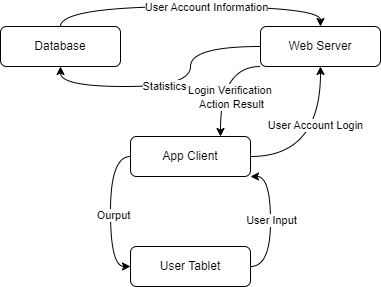
\includegraphics[width=0.7\linewidth]{Context Diagram.drawio.png} 
    \caption{Context Diagram}
\end{figure}

\subsection{Specifying a Business Use Case (BUC)}
\begin{itemize}
    \item \textbf{BUC Name:} Integrated Study Management
    \item \textbf{Goal:} To provide a comprehensive solution that allows students to manage their academic tasks, schedules, and study sessions effectively.
    \item \textbf{Actors:} Students, Educational Institutions, Teachers.
    \item \textbf{Preconditions:} User registration and course information uploaded or inputted.
    \item \textbf{Postconditions:} Enhanced student learning experiences, improved academic performance, reduced stress levels.
    \item \textbf{Main Success Scenario:} Students effectively use the app to manage their study tasks, leading to improved academic outcomes and reduced stress. Educational institutions and teachers observe enhanced student management skills and learning experiences.
    \item \textbf{Extensions:} Development of additional features based on user's feedback, improvement of machine learning model, larger user base.
\end{itemize}

\section{Business Data Model and Data Dictionary}
\subsection{Business Data Model}
\begin{figure}[htbp]
  \centering
  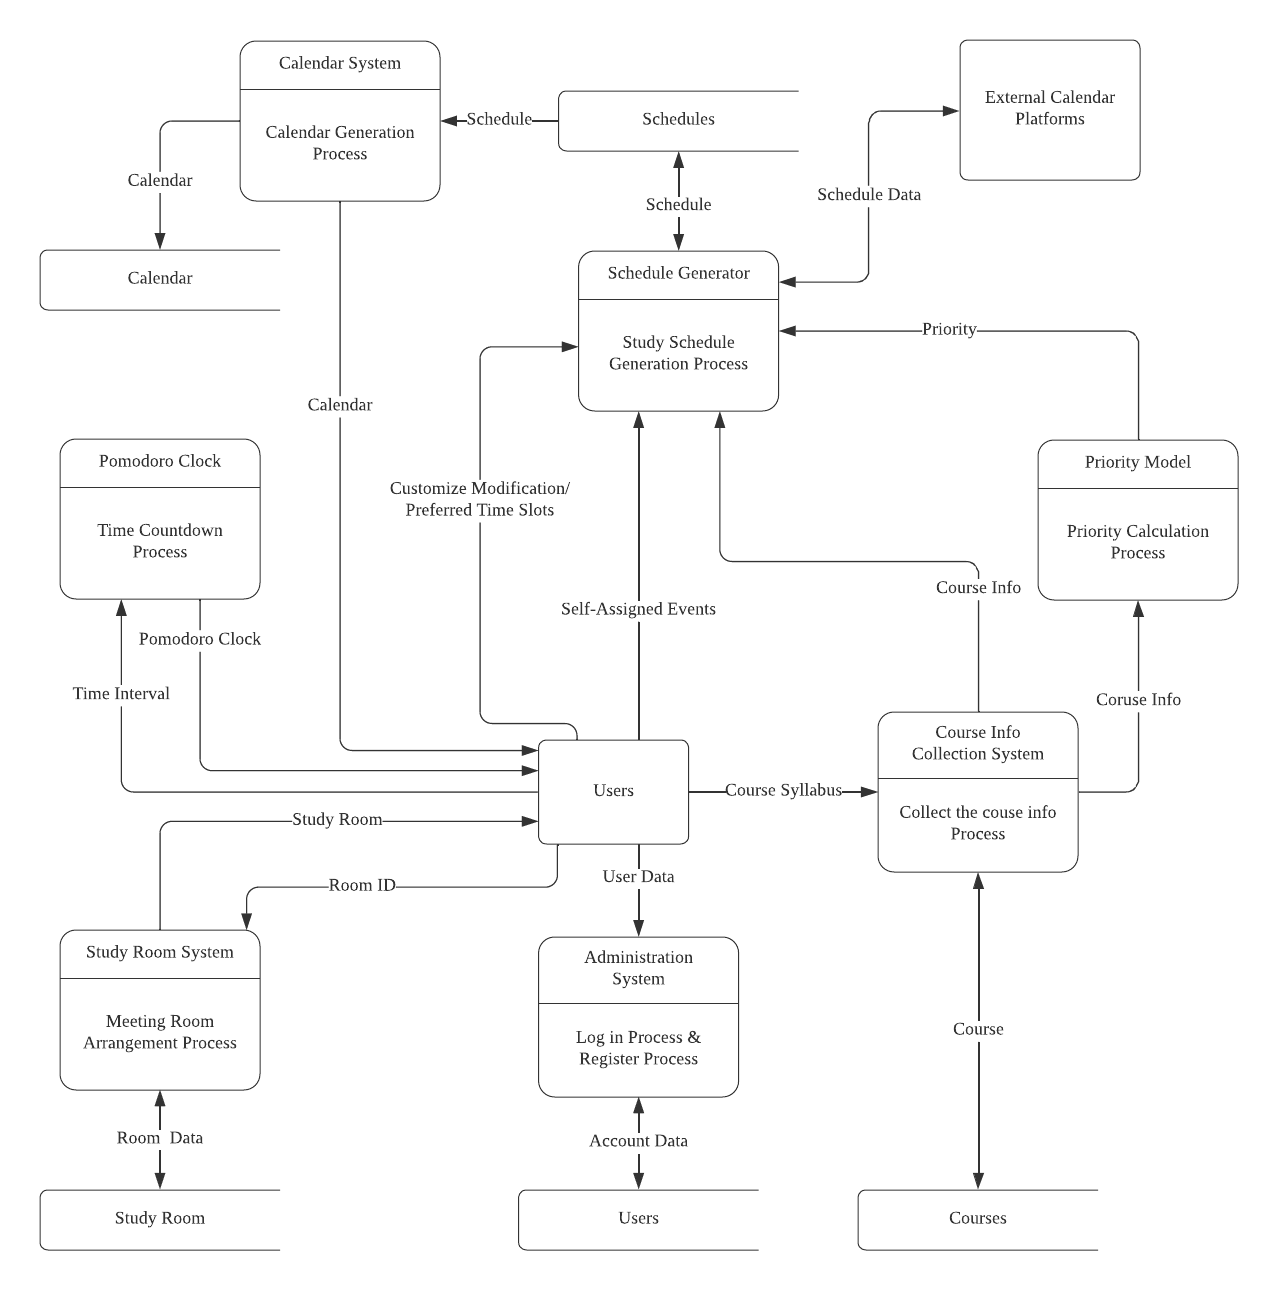
\includegraphics[width=1.2\textwidth]{DFD.png}
  \caption{Data Flow Diagram} 
  \label{fig:dfd} 
\end{figure}

\subsection{Data Dictionary}
\subsubsection{Users}

\begin{longtable}{ |p{3cm}|p{5cm}|p{5cm}|}
\hline
\multicolumn{3}{|c|}{Users} \\
\hline
Attribute & userName & userPwd \\
\hline
Description & Unique identifier of a user & The password of an account\\
\hline
Type & \texttt{VARCHAR(50)}& \texttt{VARCHAR(50)}\\
\hline
Allowed Values &N/A &N/A\\
\hline
Default Value &N/A &N/A\\
\hline
Constraints & \texttt{PRIMARY KEY, NOT NULL} & \texttt{NOT NULL CHECK (CHAR\_LENGTH(userPwd) \textgreater 8)}\\
\hline
Source & User input when setting up the account & User input when setting up the account \\
\hline
Usage & Authentication & Authentication \\
\hline
Attribute & pInterval & \\
\hline
Description & preferred Pomodoro interval & \\
\hline
Type & \texttt{INT}& \\
\hline
Allowed Values &N/A &\\
\hline
Default Value &N/A &\\
\hline
Constraints & \texttt{NOT NULL CHECK (pInterval >= 0 AND pInterval <= 300)} & \\
\hline
Source & User input when setting up the account &  \\
\hline
Usage & Scheduling &  \\
\hline
\end{longtable}
\subsubsection{Courses}
\begin{longtable}{ |p{3cm}|p{5cm}|p{5cm}|  }
\hline
\multicolumn{3}{|c|}{Courses} \\
\hline
Attribute & subject & courseCode\\
\hline
Description & The subject of a course& The code of a course\\
\hline
Type & \texttt{VARCHAR(16)}& \texttt{VARCHAR(16)}\\
\hline
Allowed Values &N/A &N/A\\
\hline
Default Value &N/A &N/A\\
\hline
Constraints & \texttt{NOT NULL, PART OF PRIMARY KEY}& \texttt{NOT NULL, PART OF PRIMARY KEY}\\
\hline
Source & Extracted from the course outline & Extracted from the course outline\\
\hline
Usage & Record course information & Record course information\\
\hline
Attribute & courseId&\\
\hline
Description & The unique identifier of a course&\\
\hline
Type & \texttt{VARCHAR(16)}&\\
\hline
Allowed Values & N/A&\\
\hline
Default Value &N/A &\\
\hline
Constraints & \texttt{PRIMARY KEY}&\\
\hline
Source & Uniquely generated when a course outline is uploaded&\\
\hline
Usage & Record course information &\\
\hline
\end{longtable}

\subsubsection{Tasks}
\begin{longtable}[H]{ |p{3cm}|p{5cm}|p{5cm}|  }
\hline
\multicolumn{3}{|c|}{Tasks} \\
\hline
Attribute & weight & taskType\\
\hline
Description & The percentage weight associated with a task & The type of a task\\
\hline
Type & \texttt{DECIMAL(10,2)}& \texttt{INT}\\
\hline
Allowed Values &N/A & \parbox{5cm}{\texttt{0 - QUIZ}\\ \texttt{1 - ASSIGNMENT}\\ \texttt{2 - PRESENTATION}\\ \texttt{3 - MIDTERM}\\ \texttt{4 - EXAM}\\ \texttt{5 - REPORT}\\ \texttt{6 - OTHER}} \\
\hline
Default Value & 0& 0\\
\hline
Constraints & \texttt{NOT NULL CHECK (weight >= 0 AND weight <= 100)}& \texttt{NOT NULL}\\
\hline
Source & Extracted from the course outline & Extracted from the course outline \\
\hline
Usage & Record course information  & Record course information \\
\hline
Attribute & subject & courseCode\\
\hline
Description & The subject of a course& The code of a course\\
\hline
Type & \texttt{VARCHAR(16)}& \texttt{VARCHAR(16)}\\
\hline
Allowed Values &N/A &N/A\\
\hline
Default Value &N/A &N/A\\
\hline
Constraints & \texttt{NOT NULL}& \texttt{NOT NULL}\\
\hline
Source & Extracted from the course outline & Extracted from the course outline\\
\hline
Usage & Record course information & Record course information\\
\hline
Attribute & courseId&priority\\
\hline
Description & The unique identifier of a course & The priority ranking of a task\\
\hline
Type & \texttt{VARCHAR(16)}&INT\\
\hline
Allowed Values &N/A &N/A\\
\hline
Default Value &N/A &0\\
\hline
Constraints & \texttt{NOT NULL}&\texttt{NOT NULL}\\
\hline
Source & Uniquely generated when a course outline is uploaded&Calculated with \texttt{weight, deadline} and taskType\\
\hline
Usage & Record course information & Record priority of a task.\\
\hline
Attribute & deadline&\\
\hline
Description & The deadline of a task & \\
\hline
Type & \texttt{DATE}&\\
\hline
Allowed Values &N/A &\\
\hline
Default Value &N/A &\\
\hline
Constraints & \texttt{NOT NULL}&\\
\hline
Source & Extracted from the course outline&\\
\hline
Usage & Record course information & \\
\hline
\end{longtable}


\section{The Scope of the Product}

\subsection{Product Boundary}
The Smart Study Helper App aims to serve as a comprehensive solution for students to manage their study schedules and tasks effectively. Its boundary extends from user registration, task generation, and prioritization, to progress visualization and study planning. It will interact with external calendar services and will allow users to collaborate with peers through its social network component. However, the app’s boundary does not extend to managing non-academic tasks or any other aspects of a user’s daily life not related to their study.

\subsection{Product Use Case Table}
\begin{longtable}{ |p{3cm}|p{5cm}|p{5cm}|}
    \hline
    Use Case Name & Primary Actor & Description \\
    \hline
    User Registration & Student & Allows new users to create an account \\
    \hline
    Upload Syllabus & Student & Enables users to upload course syllabus in PDF format \\
    \hline
    Task Generation & Application & Automatically generates tasks based on uploaded syllabus \\
    \hline
    Task Prioritization & Application & Prioritizes tasks based on ML algorithms \\
    \hline
    Progress Visualization & Student & Users can view the status of their tasks \\
    \hline
    Facial Recognition & Application & Detect users' stress levels by recognizing users' face \\
    \hline
    Classmates Lookup & Student & Users can look up online classmates who register the same course \\
    \hline
    Connected Learning & Student & Users can connect with their friends or classmates to study together \\
    \hline
    User Login & Student & Allows users to log into their accounts using username and password \\
    \hline
    Friend List Management & Student & Supports friend list for sending/rejecting/accepting friend requests \\
    \hline
    Export to Other Calendars & Application, Student & Exports event and schedule data to third-party calendar apps \\
    \hline
    Estimate Task Duration & Application & Calculates the estimated time for each task from course outlines \\
    \hline
\end{longtable}

\subsection{Individual Product Use Cases (PUC’s)}
\begin{figure}[htbp]
    \centering
    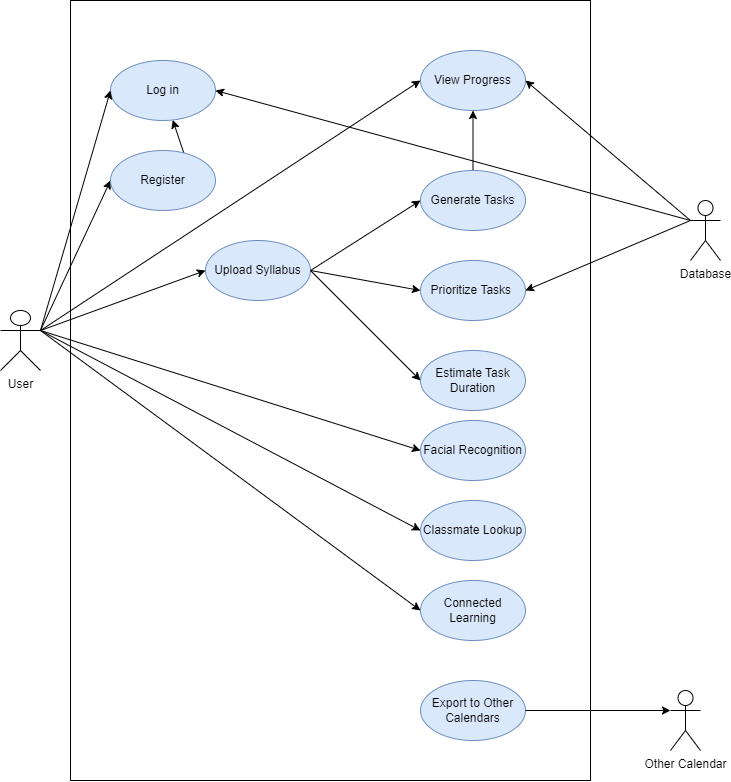
\includegraphics[width=1.0\linewidth]{Use Case Diagram.drawio.png} 
    \caption{Use Case Diagram}
\end{figure}

\subsubsection{User Registration}
\begin{itemize}
    \item \textbf{Goal:} Enable students to create a unique account.
    \item \textbf{Actors:} Student.
    \item \textbf{Preconditions:} Student has accessed the application or web.
    \item \textbf{Postconditions:} Student has an active account and can access the app's features.
    \item \textbf{Main Flow:} Student enters required information, sets a password, and completes registration.
\end{itemize}

\subsubsection{Upload Syllabus}
\begin{itemize}
    \item \textbf{Goal:} Allow students to upload their course syllabus.
    \item \textbf{Actors:} Student.
    \item \textbf{Preconditions:} Student is logged in.
    \item \textbf{Postconditions:} Syllabus is stored and ready for task generation.
    \item \textbf{Main Flow:} Student selects the course syllabus in PDF format and uploads it.
\end{itemize}

\subsubsection{Task Generation}
\begin{itemize}
    \item \textbf{Goal:} Create tasks from the uploaded syllabus.
    \item \textbf{Actors:} Application.
    \item \textbf{Preconditions:} Syllabus has been uploaded.
    \item \textbf{Postconditions:} Tasks are generated and displayed to the student.
    \item \textbf{Main Flow:} Application processes the syllabus and generates relevant tasks.
\end{itemize}

\subsubsection{Task Prioritization}
\begin{itemize}
    \item \textbf{Goal:} Rank tasks based on importance.
    \item \textbf{Actors:} Application.
    \item \textbf{Preconditions:} Tasks have been generated.
    \item \textbf{Postconditions:} Tasks are prioritized and presented in an organized manner.
    \item \textbf{Main Flow:} Application uses ML algorithms to analyze and prioritize tasks.
\end{itemize}

\subsubsection{Progress Visualization}
\begin{itemize}
    \item \textbf{Goal:} Offer students a view of their task progress.
    \item \textbf{Actors:} Student.
    \item \textbf{Preconditions:} Tasks have been generated and prioritized.
    \item \textbf{Postconditions:} Student can visually assess task status.
    \item \textbf{Main Flow:} Student accesses a dashboard or progress section to view status of tasks.
\end{itemize}

\subsubsection{Facial Recognition}
\begin{itemize}
    \item \textbf{Goal:} Identify student stress levels using facial cues.
    \item \textbf{Actors:} Application.
    \item \textbf{Preconditions:} Student grants camera access.
    \item \textbf{Postconditions:} App detects potential stress indicators.
    \item \textbf{Main Flow:} Application uses facial recognition technology to analyze student's face for stress signs.
\end{itemize}

\subsubsection{Classmates Lookup}
\begin{itemize}
    \item \textbf{Goal:} Allow students to find classmates in the same course.
    \item \textbf{Actors:} Student.
    \item \textbf{Preconditions:} Student is registered in a course.
    \item \textbf{Postconditions:} Student views a list of classmates in the same course.
    \item \textbf{Main Flow:} Student accesses course section and views registered classmates.
\end{itemize}

\subsubsection{Connected Learning}
\begin{itemize}
    \item \textbf{Goal:} Provide students with a platform to study collaboratively.
    \item \textbf{Actors:} Students.
    \item \textbf{Preconditions:} Students have active accounts.
    \item \textbf{Postconditions:} Students can connect and study together.
    \item \textbf{Main Flow:} A student sends a connection request to another student. Once accepted, they can access video chat with joint study tools and features.
\end{itemize}

\subsubsection{User Login}
\begin{itemize}
    \item \textbf{Goal:} Allow students to log into their account.
    \item \textbf{Actors:} Student.
    \item \textbf{Preconditions:} Student has an active account.
    \item \textbf{Postconditions:} Student is logged in and can access personalized data.
    \item \textbf{Main Flow:} Student provides username and password; if credentials match, access is granted.
\end{itemize}

\subsubsection{Friend List Management}
\begin{itemize}
    \item \textbf{Goal:} Manage friend connections within the application.
    \item \textbf{Actors:} Student.
    \item \textbf{Preconditions:} Student is logged in.
    \item \textbf{Postconditions:} Updated friend list status (friend request sent/received/accepted/rejected).
    \item \textbf{Main Flow:} Student navigates to the friend list section, sends/receives/accepts/rejects friend requests.
\end{itemize}

\subsubsection{Export to Other Calendars}
\begin{itemize}
    \item \textbf{Goal:} Export event and schedule data to third-party calendar apps.
    \item \textbf{Actors:} Application, Student.
    \item \textbf{Preconditions:} Student has events or schedules in the application.
    \item \textbf{Postconditions:} Events and schedules are exported and viewable in third-party apps.
    \item \textbf{Main Flow:} With authentication, the student initiates export to a chosen calendar app; data is formatted and transferred.
\end{itemize}

\subsubsection{Estimate Task Duration}
\begin{itemize}
    \item \textbf{Goal:} Calculate the estimated time needed for each task from course outlines.
    \item \textbf{Actors:} Application.
    \item \textbf{Preconditions:} Tasks have been extracted from course outlines.
    \item \textbf{Postconditions:} Each task has an associated time estimate.
    \item \textbf{Main Flow:} Application processes tasks from course outlines and estimates time requirements for each.
\end{itemize}


\section{Functional Requirements}
\subsection{Authentication}
\begin{itemize}[leftmargin=16.5mm,labelsep=4mm,label=\rthereqnum]

\item
The user could create an account with a username and a password.

\textbf{Rationale:} Users would need an account protected by a password to keep their schedule personal and private.

\textbf{Priority:} HIGH
\item
The user could log in to their account by providing a corresponding username and password.

\textbf{Rationale:} Users would need to access their accounts.

\textbf{Priority:} HIGH
\item
The user should be able to log out of the account.

\textbf{Rationale:} Users do not have to stay logged in.

\textbf{Priority:} HIGH
\item
The user should have access to their scheduling information once logged in.

\textbf{Rationale:} User's scheduling information should be available to them.

\textbf{Priority:} HIGH

\end{itemize}


\subsection{User input}
\begin{itemize}[leftmargin=16.5mm,labelsep=4mm,label=\rthereqnum]

\item[\rthereqnum \label{R_upload_pdf}]
The user could upload multiple PDF files containing course outlines to the system.

\textbf{Rationale:} Multiple courses would have multiple course outlines.

\textbf{Priority:} HIGH
\item
The system prompts users to choose their preferred study interval at which the system tends to allocate study sessions.

\textbf{Rationale:} The user would want to have their study session schedules at their preferred time.

\textbf{Priority:} MEDIUM
\item
The user could change their preferred study interval.

\textbf{Rationale:} The user's preferred study interval could change over time. 

\textbf{Priority:} MEDIUM
\item
The system prompts users to set their preferred Pomodoro intervals. 

\textbf{Rationale:} The user might have preferred Pomodoro intervals.

\textbf{Priority:} MEDIUM
\item
The user could change their Pomodoro interval.

\textbf{Rationale:} The user's preferred Pomodoro intervals could change over time.

\textbf{Priority:} MEDIUM
\item
The system supports a friend list allowing users to send friend requests.

\textbf{Rationale:} The user needs to send friend requests to add friends.

\textbf{Priority:} LOW
\item
The user could accept an incoming friend request.

\textbf{Rationale:} The user could accept the friend request if they wish to befriend the request sender.

\textbf{Priority:} LOW
\item
The user could reject an incoming friend request.

\textbf{Rationale:} The user could reject the friend request if they wish not to befriend the request sender.

\textbf{Priority:} LOW
\item
The user could change the progress of each task

\textbf{Rationale:} The progress of each task should align with reality.

\textbf{Priority:} HIGH
\item
On finishing each sub-task, the system should ask for the user's feedback on whether the pace is comfortable.

\textbf{Rationale:} The schedule needs feedback to adjust the pace.

\textbf{Priority:} HIGH
\end{itemize}

\subsection{Data}
\begin{itemize}[leftmargin=16.5mm,labelsep=4mm,label=\rthereqnum]
\item
The system could extract information including \texttt{courseName, taskType, taskName, weight, deadline} from the uploaded course outline PDF files.

\textbf{Rationale:} Course outlines would be provided as PDF files containing course information.

\textbf{Priority:} HIGH
\item
The system could generate a list of tasks from uploaded PDFs.

\textbf{Rationale:} To generate a study plan, tasks to be finished are needed.

\textbf{Priority:} HIGH
\item[\rthereqnum \label{R_prioritize_task}]
The system could assign priority to each task generated.

\textbf{Rationale:} From priority the system could allocate adequate time to finish each task.

\textbf{Priority:} HIGH
\item
The system could detect the user's attention level.

\textbf{Rationale:} The user's attention level is needed to allocate rest time.

\textbf{Priority:} MEDIUM
\item
The system should notify the user when the user's attention level is low.

\textbf{Rationale:} The system would keep the user engaged in their study task.

\textbf{Priority:} MEDIUM
\item[\rthereqnum \label{R_check_task_progress}]
The user should be able to view the progress of each task.

\textbf{Rationale:} The user would want to see their progress.

\textbf{Priority:} HIGH
\item
With authentication, the system could import event and schedule data from other calendar apps including Calendar, Outlook, and Google Calendar.

\textbf{Rationale:} Study session allocation would consider avoiding conflicts with existing events.

\textbf{Priority:} MEDIUM
\item
With authentication, the system could export event and schedule data to other calendar apps including Calendar, Outlook, and Google Calendar.

\textbf{Rationale:} The user would want to use their own calendar of choice.

\textbf{Priority:} MEDIUM
\item
The user should be able to export their study plan as a PDF.

\textbf{Rationale:} The user could want to have an overview of their study plan offline.

\textbf{Priority:} LOW
\end{itemize}

\subsection{Scheduling}
\begin{itemize}[leftmargin=16.5mm,labelsep=4mm,label=\rthereqnum]
\item
The system could calculate the estimated time needed to finish each task. 

\textbf{Rationale:} Total required tie is needed to decide the amount of subtasks needed.

\textbf{Priority:} HIGH
\item
The user could regenerate a study plan accordingly once a task's progress is changed by the user.

\textbf{Rationale:} Previously generated study plans could be outdated.

\textbf{Priority:} HIGH
\item
The estimated time needed to finish each task would dynamically adjust based on user feedback on past task completion progress.

\textbf{Rationale:} Estimated time needed may not be perfect.

\textbf{Priority:} HIGH
\item
The system could prioritize tasks extracted based on \texttt{taskType, weight} and \texttt{deadline}.

\textbf{Rationale:} The system would ensure high-priority tasks are finished on time.

\textbf{Priority:} HIGH
\item
With data containing task information, preferred study time, schedule, and Pomodoro intervals gathered the system could generate a detailed study plan containing multiple sub-tasks for each task in the course outline available in-app and export it to other calendars.

\textbf{Rationale:} A detailed study plan contains all the sub-tasks and their settings.

\textbf{Priority:} HIGH
\item
The system would have a Pomodoro clock ready for each sub-task.

\textbf{Rationale:} A Pomodoro clock would help the user balance their study and rest.

\textbf{Priority:} MEDIUM
\item
With a detailed study plan, the system could pair friends from the friend list with similar study plans to have video-based online study sessions.

\textbf{Rationale:} Friends with similar tasks at similar times could collaborate and inspire each other.

\textbf{Priority:} LOW
\end{itemize}
\section{Look and Feel Requirements}

\subsection{Appearance Requirements}
The application's design should be user-friendly and intuitive. Key elements to consider include:
\paragraph{AR1:} Clear typography: Text should be legible at all standard screen resolutions and sizes. 
\paragraph{AR2:}Color scheme: The color palette should be eye-catching but not overwhelming. Calming and neutral tones should be used that helps to focus.
\paragraph{AR3:}Icons and graphics: Visual aids should be recognizable and easy to learn.
\paragraph{AR4:}Layout: The design should be responsive, ensuring usability across devices of varying screen sizes, from smartphones to tablets to desktop monitors.

\subsection{Style Requirements}
The style of the application should make the application easy and clear to use, providing a sense of community for students. Aspects to focus on include:
\paragraph{SR1:}Navigation: Menus and navigation tools should be logically organized and easy to access. 
\paragraph{SR2:}Consistency: Elements like buttons, text fields, and icons should maintain a consistent design throughout the application.
\paragraph{SR3:}Interactivity: Interactive elements like buttons or dropdowns should provide feedback, indicating appropriate responsiveness.
\paragraph{SR4:}Accessibility: The design should cater to all users, including those with disabilities and elder adults. Features like text-to-speech and adjustable font sizes should be considered.
\paragraph{SR5:}Animations: Any animations used should be subtle and not distractive so users can focus more on the main content. 



\section{Usability and Humanity Requirements}
\subsection{Ease of Use Requirements}
\begin{itemize}[leftmargin=16.5mm,labelsep=4mm,label=\rtheuhrnum]
\item The navigation must be intuitive to use by users with \texttt{MIN\_EDUCATION} education background.

\textbf{Fit Criterion:} \texttt{MIN\_UNDERSTAND\%} of users with at least \texttt{MIN\_EDUCATION} of education could navigate through functions within \texttt{MAX\_TRIAL\_TIME} of exploring.

\begin{itemize}
    \item \( U \): Total number of users
    \item \( E \): The set of users with at least \texttt{MIN\_EDUCATION}
    \item \( N \): The number of users who can navigate through functions within \texttt{MAX\_TRIAL\_TIME}
\end{itemize}
\[
    N \geq \left( \frac{\texttt{MIN\_UNDERSTAND\%}}{100} \right) \cdot |E|
\]
\end{itemize}
\subsection{Personalization and Internationalization Requirements}
N/A
\subsection{Learning Requirements}
\begin{itemize}[leftmargin=16.5mm,labelsep=4mm,label=\rtheuhrnum]
\item
The system must be understood by users within \texttt{MAX\_TRIAL\_TIME} of exploring.

\textbf{Fit Criterion:} \texttt{MIN\_UNDERSTAND\%} of users with at least \texttt{MIN\_EDUCATION} of education could understand the system within \texttt{MAX\_TRIAL\_TIME} of exploring.
\begin{itemize}
    \item \( U \): Total number of users
    \item \( E \): The set of users with at least \texttt{MIN\_EDUCATION}
    \item \( N \): The number of users who can navigate through functions within \texttt{MAX\_TRIAL\_TIME}
\end{itemize}

\[
    N \geq \left( \frac{\texttt{MIN\_UNDERSTAND\%}}{100} \right) \cdot |E|
\]
\end{itemize}
\subsection{Understandability and Politeness Requirements}
\begin{itemize}[leftmargin=16.5mm,labelsep=4mm,label=\rtheuhrnum]
\item
The language in the app must be grammatically correct \texttt{MIN\_grammar\%} of the time.

\textbf{Fit Criterion:} A group of \texttt{MIN\_TESTER\_NUM}  users could find at most \texttt{MAX\_BAD\_GRAMMAR} of grammar mistakes.

\item
The language in the app must be non-offensive.

\textbf{Fit Criterion:} A group of \texttt{MIN\_TESTER\_NUM} users could find no more than \texttt{MAX\_OFFENSIVE} of offensive messages.
\begin{itemize}
    \item \( U \): Total number of users testing the system
    \item \( O \): The number of offensive messages found by a group of users
    \item \( G \): The group of at least \texttt{MIN\_TESTER\_NUM} users
\end{itemize}
\[
    O \leq \texttt{MAX\_OFFENSIVE}
\]
\end{itemize}
\subsection{Accessibility Requirements}
\begin{itemize}[leftmargin=16.5mm,labelsep=4mm,label=\rtheuhrnum]
    \item Color combinations used in the interface must be distinguished by users with color blindness.\\
    
    \textbf{Fit Criterion:} A group of \texttt{MIN\_TESTER\_NUM} users could find at most \texttt{MAX\_COLOR\_AMBIGUOUS} of indistinguishable color combinations in the UI filtered with Color Oracle.
    \begin{itemize}
        \item \( C \): The number of indistinguishable color combinations found by a group of users, filtered with Color Oracle
        \item \( G \): The group of at least \texttt{MIN\_TESTER\_NUM} users
    \end{itemize}
    \[
        C \leq \texttt{MAX\_COLOR\_AMBIGUOUS}
    \]
\end{itemize}
\section{Performance Requirements}

\subsection{Speed and Latency Requirements}
\paragraph{SLR1:} Major actions, such as uploading syllabuses, generating tasks, and prioritizing tasks, should be completed in a timely manner.
\paragraph{Fit Criteria:} During testing under normal load conditions, major actions are executed within a 2-second threshold.

\subsection{Safety-Critical Requirements}
\paragraph{SCR1:} All data, especially sensitive academic information, must be securely encrypted to ensure protection against unauthorized access.
\paragraph{Fit Criteria:} Throughout security testing, no incidents of data breaches or unauthorized data accesses are observed.

\subsection{Precision or Accuracy Requirements}
\paragraph{PAR1:} ML-based features, particularly task prioritization, must achieve a high degree of accuracy.
\paragraph{Fit Criteria:} When tested against predefined scenarios, ML algorithms show an accuracy rate of 90\% in task categorization and prioritization.

\subsection{Robustness or Fault-Tolerance Requirements}
\paragraph{RFTR1:} The application must demonstrate resilience against unexpected inputs or actions and provide means of efficient data recovery.


\subsection{Capacity Requirements}
\paragraph{CR1:} The system should be robust enough to manage a large number of concurrent users.
\paragraph{Fit Criteria:} During load testing, the application manages the equivalent load of 10,000 users and data pertaining to 1 million courses without any performance issues or system crashes.
\paragraph{CR2:}The system should store vast quantities of course data without any compromise in performance.
\paragraph{Fit Criteria:} During load testing, the application manages the equivalent load of 1 million courses without any performance issues or system crashes.
\subsection{Scalability or Extensibility Requirements}
\paragraph{SER1:} The design and architecture of the application should support ease of modification and the addition of new features.
\subsection{Longevity Requirements}
N/A

\section{Operational and Environmental Requirements}
\subsection{Expected Physical Environment}
\begin{itemize}[leftmargin=16.5mm,labelsep=4mm,label=\rtheoernum]
\item
The system must be operable under the same physical environment that the desktop computer running it is operable.

\textbf{Fit Criterion:} When the machine is operable, the system is operable at least \texttt{MIN\_OPERABLE\%} of time.
\begin{itemize}
    \item \( T \): Total time the machine is operable
    \item \( S \): Total time the system is operable when the machine is operable
\end{itemize}
\[
    \frac{S}{T} \geq \frac{\texttt{MIN\_OPERABLE\%}}{100}
\]
\end{itemize}
\subsection{Requirements for Interfacing with Adjacent Systems}
\begin{itemize}[leftmargin=16.5mm,labelsep=4mm,label=\rtheoernum]
\item
The system could interface with calendar APIs when called.

\textbf{Fit Criterion:} At least \texttt{MIN\_API\_SUCCESS\%} of requests made to supported calendar APIs are successful.
\begin{itemize}
    \item \( R \): Total number of requests made to the supported calendar APIs
    \item \( S \): Number of successful requests made to the supported calendar APIs
\end{itemize}
\[
    \frac{S}{R} \geq \frac{\texttt{MIN\_API\_SUCCESS\%}}{100}
\]
\end{itemize}
\subsection{Productization Requirements}
N/A
\subsection{Release Requirements}
\begin{itemize}[leftmargin=16.5mm,labelsep=4mm,label=\rtheoernum]
\item
The released version must pass all known regression tests.

\textbf{Fit Criterion:} The released version must pass \texttt{MIN\_REGRESSION\_PASS\%} of regression tests. 
\begin{itemize}
    \item \( T \): Total number of regression tests conducted on the released version
    \item \( P \): Number of regression tests passed by the released version
\end{itemize}
\[
    \frac{P}{T} \geq \frac{\texttt{MIN\_REGRESSION\_PASS\%}}{100}
\]
\end{itemize}

\section{Maintainability and Support Requirements}
\subsection{Maintenance Requirements}

\begin{itemize}[leftmargin=14.5mm,labelsep=4mm,label=\rthemreqnum]
    \item The bugs and issues should be addressed within a response time corresponding to their severity. \\
    \textbf{Fit Criteria}: If a bug significantly impacts the regular user experience, the response time for resolution does not exceed \texttt{MAX\_RESPONSE\_TIME} hours.
    \item The updates and patches should be delivered periodically.\\
    \textbf{Fit Criteria}: A feature update, aligned with user preferences and market trends, can be released each season.
    \item The application should be documented comprehensively, with a user manual, technical report, and clear code comments for further navigation and maintenance.\\
    \textbf{Fit Criteria}: A user manual can provide tutorials for full product feature utilization. A technical report should be updated at least once every season's maintenance. Clear code comments should be provided to facilitate developers’ navigation and maintenance.

\end{itemize}

\subsection{Supportability Requirements}
\begin{itemize}[leftmargin=13mm,labelsep=4mm,label=\rthesreqnum]
    \item Users shall have easy access to a helpdesk for support.\\
    \textbf{Fit Criteria}: Users are able to access the email contact, phone contact, and chatbot to address common user questions in \texttt{MAX\_SUPPORT\_STEP} steps.\\
    \item The response time for offering support should be on time corresponding to the support type. \\
    \textbf{Fit Criteria}: For critical functionality disasters, the support should be delivered within \texttt{MAX\_RESPONSE\_TIME} hours.\\
    \item The application should have a mechanism for collecting users’ feedback for product continuous improvement.\\
    \textbf{Fit Criteria}: Users are able to provide feedback when they want.\\

\end{itemize}
\subsection{Adaptability Requirements}
\begin{itemize}[leftmargin=14mm,labelsep=4mm,label=\rtheareqnum]
    \item The product should be compatible with common systems and \textit{API}s to facilitate seamless integration and data exchange. \\
    \textbf{Fit Criteria}: The product can interact with the \textit{Google} \textit{Calendar} \textit{API} through explicit \textit{HTTP} calls or using the \textit{Google} \textit{Client} \textit{Libraries}. \\
    \item The product should implement modular architecture, allowing for the addition or replacement of components without causing issues.\\
    \textbf{Fit Criteria}: The products’ independent modules can interact with each other through de-coupled interfaces.\\
\end{itemize}

\section{Security Requirements}
\subsection{Access Requirements}
\begin{itemize}[leftmargin=13.5mm,labelsep=4mm,label=\rthesrnum]
\item
The system is accessible only if the correct combo of username and password is provided.

\textbf{Fit Criterion:} An error message suggesting an incorrect password or username is displayed.
\item
Users could not access other users' data.

\textbf{Fit Criterion:} Only data linked to the currently logged-in account could be displayed.
\end{itemize}
\subsection{Integrity Requirements}
\begin{itemize}[leftmargin=13.5mm,labelsep=4mm,label=\rthesrnum]
\item
No Unauthorised entity could modify the database.

\textbf{Fit Criterion:} A group of \texttt{MIN\_TESTER\_NUM} unauthorised users could not modify data.
\end{itemize}
\subsection{Privacy Requirements}
\begin{itemize}[leftmargin=13.5mm,labelsep=4mm,label=\rthesrnum]
\item
The system will not release user information to a third party.

\textbf{Fit Criterion:} The system does not provide user information to a third party.
\end{itemize}
\subsection{Audit Requirements}
N/A
\subsection{Immunity Requirements}
N/A

\section{Cultural Requirements}
\subsection{Cultural Requirements}
\begin{itemize}[leftmargin=13.5mm,labelsep=4mm,label=\rthecreqnum]
    \item The application shall be easily translatable into various languages without causing ambiguity in meaning.\\
    \textbf{Fit Criteria}: The application can be translated into at least \texttt{MIN\_LANGUAGE} languages(Spanish, French, Chinese, Italian and German).\\
    \item The product shall avoid elements such as confusing icons, symbols, or offensive images that might cause controversy in different cultural environments.\\
    \textbf{Fit Criteria}: Users are able to feel comfortable and respected.\\
\end{itemize}

\section{Compliance Requirements}
\subsection{Legal Requirements}
\begin{itemize}[leftmargin=16.5mm,labelsep=4mm,label=\rthecprnum]
\item The system must comply with local laws and regulations.

\textbf{Fit Criterion:} The system does not violate local laws or regulations.
\end{itemize}
\subsection{Standards Compliance Requirements}
\begin{itemize}[leftmargin=16.5mm,labelsep=4mm,label=\rthecprnum]
\item The code must comply with \textit{Flack8} coding standards.

\textbf{Fit Criterion:} Merged code passes \textit{Flake8} linter workflow check.
\end{itemize}

\section{Open Issues}
 The application features should identify the dependency relationships for better organizing the development process.\\


\section{Off-the-Shelf Solutions}
\subsection{Ready-Made Products}

    The off-the-shelf product should be compatible with our application currently using technology stack, infrastructure and operating system (\textit{Windows} or \textit{IOS}, excluding \textit{Linux}).
    Also, the selection of ready-made products shall be based on cost-effectiveness and alignment with the project's functionality requirements.
    
\subsection{Reusable Components}
For text and PDF extraction, reusable components could include robust text parsing algorithms, and document structure analysis tools, which can be used across various document types. In the context of modelling, reusable components could consist of machine learning models that have been trained on diverse datasets. Furthermore, in the field of facial recognition, reusable components may encompass pre-trained facial detection models and privacy protection mechanisms. Also, some existing website extensions or components can also be reused to assist the application development. \\
\subsection{Products That Can Be Copied}
The configuration location and integrated module should be clearly defined in the documentation, also developer should maintain records of the updated versions of the copied source product.\\


\section{New Problems}
\subsection{Effects on the Current Environment}

\begin{itemize}
    \item The implementation of a new system may change the way students interact with existing tools and platforms. If the new tool enables integration with existing popular scheduling platforms, users may stop using other scheduling tools. Some users may need to adapt to these changes, and this transition needs to be handled carefully to ensure a smooth user experience.

    \item The data security requirements of the new tool and the user access control may require changes to the current security infrastructure. Any potential impact on existing security protocols should be fully assessed, and measures taken to mitigate risks.

    \item The new system may change user workflows and procedures. If it automates and prioritizes tasks, this may impact the way they plan and manage assignment completion and course scheduling. Understanding and responding to these changes as early as possible is critical to ensure smooth operation.
\end{itemize}

\subsection{Effects on the Installed Systems}
This section specifies the interfaces between the new system and existing systems or components.
\begin{itemize}
    \item \textbf{Interface with Google Calendar}: The system should integrate with Google Calendar to synchronize and visualize task deadlines. The interface will involve certification, data exchange, and event management.
    
    \item \textbf{Interface with Outlook Calendar}: Similar to Google Calendar, the system shall integrate with Outlook Calendar to synchronize events. The interface will involve certification and event management.

    \item \textbf{Interface with Machine Learning Server}: The system relies on machine learning algorithms to prioritize tasks. This interface includes sending data to the machine learning server, processing suggestions, and integrating them into the user interface.

    \item \textbf{Interface to connect with users}: To facilitate collaborative learning, the system should enable users to connect with their peers. This interface includes user authentication, data exchange, and video chat integration.

    \item \textbf{Interface with videoconferencing hardware} Users will use webcams, microphones, and speakers for video chat during collaborative learning. This interface is required to access these hardware components and manage live video conferencing.
\end{itemize}
\subsection{Potential User Problems}
\begin{itemize}
    \item \textbf{User Confusion}:
    The addition of machine learning-driven task prioritization, facial recognition, and online collaborative learning session features may confuse or create resistance from some users who are unfamiliar with these concepts.
    
    \textbf{Prevention and mitigation measures:}
    \begin{itemize}
        \item Develop a user-friendly onboarding process and provide extensive training materials to ensure users can easily understand and use the new features.
        \item Provide customization options that allow users to customize the system to their preferences. This flexibility will help users take better control of their experience.
    \end{itemize}
    
    \item \textbf{Privacy Concerns}:
    Users may have privacy concerns, especially with attention-monitoring features such as facial recognition. They may be concerned that their facial data will be collected and used.
    
    \textbf{Prevention and Mitigation Measures:}
    \begin{itemize}
        \item Privacy concerns are addressed by implementing strong data protection measures. Users will be informed of what their data will be used for and how it will be processed and will be able to opt out of certain features.
    \end{itemize}
    
    \item \textbf{Technical Issues}:
    Technical issues or system incompatibilities may lead to adverse reactions, such as issues related to platform support or software bugs.
    
    \textbf{Prevention and Mitigation Measures:}
    \begin{itemize}
        \item Rigorous testing and quality assurance are conducted to detect and correct technical issues before they affect users. Updates and bug fixes will be performed regularly to ensure system stability.
    \end{itemize}
\end{itemize}

\subsection{Limitations in the Anticipated Implementation Environment That May
Inhibit the New Product}
\begin{itemize}
    \item The planned servers may not have enough processing power or storage capacity to handle the expected growth in users and data volume.
    
    \item Available network bandwidth may not be sufficient to support real-time videoconferencing for collaborative learning sessions, leading to potential performance issues.
    
    \item Implementing system integration with external calendaring platforms (e.g., Google Calendar, Outlook) takes into account that these platforms may have limitations or constraints that affect the quality of the integration.
    
    \item Hardware for facial recognition may not be readily available or may not meet the accuracy requirements for detecting the user's level of attention.
    
    \item The implementation environment may be subject to specific data privacy regulations that may affect the collection and storage of user data.
\end{itemize}

\subsection{Follow-Up Problems}
This section anticipates potential challenges, unintended consequences, and limitations that the project may encounter during development and implementation.

\begin{itemize}
    \item The implementation of new features or technologies in the system may inadvertently result in non-compliance with existing laws and regulations, such as user privacy protection aspect. The project team will conduct regular assessments. Any necessary changes will be made to address potential legal issues.
\end{itemize}

\section{Tasks}
\subsection{Project Planning}
\href{https://github.com/wangq131/4G06CapstoneProjectT5/blob/main/docs/DevelopmentPlan/DevelopmentPlan.tex#L248C1-L265C6}{See Project Scheduling Section in Development Plan.}
\subsection{Planning of the Development Phases}
\href{https://github.com/wangq131/4G06CapstoneProjectT5/blob/main/docs/DevelopmentPlan/DevelopmentPlan.tex#L194C1-L245C16}{See Project Scheduling Section in Development Plan.}

\section{Migration to the New Product}
The project is a stand-alone application, not an upgrade or replacement of an existing product. There is no need to involve a product migration. The Migration to the New Product section is not needed.

\section{Costs}
The following are some of the major cost items that may need to be considered:

\begin{itemize} 
  \item \textbf{Cloud services}: using a cloud infrastructure (e.g. \textit{Amazon AWS}, \textit{Microsoft Azure}, or \textit{Google Cloud}) requires consideration of the cost of using cloud services.
  \item \textbf{Server hosting}: using an independent server, server hosting, and maintenance costs need to be considered.
  \item \textbf{Database}: database storage and access costs.
  \item \textbf{Data Backup}: regular data backup and storage costs.
  \item \textbf{Working Time}: takes NUMBER\_Of\_MEMBERS group members WORK\_HOURS a week.
\end{itemize}

\section{User Documentation and Training}
\subsection{User Documentation Requirements}

\begin{itemize}[leftmargin=16.5mm,labelsep=4mm,label=\rtheudreqnum]
\item A user manual that covers all functionalities of the website with step-by-step instructions should be provided in a digital format. The manual should be written in an easily understandable language, accompanied by illustrative diagrams. \\
\item User manual should be updated with each release to reflect any changes made. \\
\item A help/support channel should be provided so that users can ask questions and give feedback which will be taken into consideration for future developments and improvements.\\
\end{itemize}

\subsection{Training Requirements}
\begin{itemize}[leftmargin=16.5mm,labelsep=4mm,label=\rtheutreqnum]
\item A short tutorial should be provided if it is the user’s first time using the website. \\
\item A training video should be provided with demos on how to use major features of the website. \\
\item Training videos should be added or updated with each release to reflect any changes.\\
\end{itemize}

\section{Waiting Room}
\begin{itemize}
  \item Add a dark mode support for the website
  \item Add a colour blind support for the website
  \item Add sound effects to the website to make it more user friendly and interesting
  \item Implement a feature where the users are able to integrate with other popular music apps like Spotify to play their favourite playlists while studying
  \item Implement a badges or achievements system such as points for completing tasks which can make the use of the website more engaging and rewarding 
  \item Provide data analysis and insight on how the user performs within a period of time and provide feedback on how to improve their way of study
  \item Add support to other platforms such as mobile applications and desktop applications
\end{itemize}

\section{Ideas for Solution}
\subsection{Idea 1}
\textbf{Requirement}: \frref{R_upload_pdf}, The user could upload multiple PDF files containing course outlines to the system. \\
\textbf{Potential solution}: We could use a \textit{Python} web framework \textit{Flask} to set up a web app which supports accessing and uploading multiple files with PDF extensions.\\
\textbf{Advantages}: This will allow users to upload their PDF easily and more securely, and with no additional effort required for developers to implement and test these features, as \textit{Flask} has already taken care of it for us.\\
\textbf{Disadvantages}: Using \textit{Flask} to support this feature doesn't present any foreseeable disadvantages in the near future. \\

\subsection{Idea 2}
\textbf{Requirement}: \frref{R_prioritize_task}, The system could assign priority to each task generated. \\
\textbf{Potential solution}: A inference pipeline could be set up to give inference on the unclassified tasks using type of task, weight, and deadline as the inputs. The inference pipeline could use a trained model of task priority classification.\\
\textbf{Advantages}: Setting an inference pipeline could be more flexible and could potentially give better results than implementing an fixed algorithm for giving predictions. Several steps for the inference pipeline could be constructed and it will be easier to make changes once it gets set up, simply adding, changing or removing steps when there is a future requirement.\\
\textbf{Disadvantages}: There will be an overload of defining each step and connecting them. \\

\subsection{Idea 3}
\textbf{Requirement}: \frref{R_check_task_progress}, The user should be able to view the progress of each task. \\
\textbf{Potential solution}: Could implement a cloud based solution for holding and retrieving data of task, time, etc. A potential choice could be using \textit{AWS S3}\\
\textbf{Advantages}: This would allow users to check their progress of task and time in a more available, reliable, and well-managed service. The data can be well secured and can be accessed in many ways for example using \textit{AWS S3}, \textit{AWS console}, \textit{AWS Command Line}, providing multiple ways for developers to implement  \\
\textbf{Disadvantages}: There is a cost associated with it when using third party cloud services
\newpage{}
\section*{Appendix --- Reflection}

The information in this section will be used to evaluate the team members on the
graduate attribute of Lifelong Learning.  Please answer the following questions:

\begin{enumerate}
  \item What knowledge and skills will the team collectively need to acquire to
  successfully complete this capstone project?  Examples of possible knowledge
  to acquire include domain specific knowledge from the domain of your
  application, or software engineering knowledge, mechatronics knowledge or
  computer science knowledge.  Skills may be related to technology, or writing,
  or presentation, or team management, etc.  You should look to identify at
  least one item for each team member. \\
  
  The following knowledge and skills will the team need to acquire to successfully complete this capstone project:
  \begin{itemize}
    \item GitHub features such as issue tracker, using workflows/\textit{Github Actions}, setting up \textit{Dev Containers}, etc.
    \item Machine learning and neural network knowledge for the developing and optimizing task priority classification models
    \item Machine learning libraries and frameworks such as \textit{pandas}, \textit{scikit-learn}, and \textit{Keras}
    \item \textit{Python} web framework for web development such \textit{Streamlit} and \textit{Flask}
    \item Agile methodologies such as sprint planning and for team management, efficient collaborations and constant delivery, which is important for incremental and iterative development like this project
  \end{itemize}
  \item For each of the knowledge areas and skills identified in the previous
  question, what are at least two approaches to acquiring the knowledge or
  mastering the skill?  Of the identified approaches, which will each team
  member pursue, and why did they make this choice?
  \begin{table}[]
    \begin{tabular}{| p{3cm} | p{3.5cm} | p{2cm} | p{5cm} |}
    \hline
      \textbf{Knowledge or Skills} & \textbf{Approaches} & \textbf{Assigned Team Member} & \textbf{Reason} \\
    \hline
      GitHub & \raggedright Use \textit{ChatGPT}, \texit{Google}, watch online tutorials, or ask supervisor for help  & Shuting, Shi & Strong interest in using \textit{GitHub} for project management, previous experience with other projects. \\
    \hline
      \raggedright Machine learning and neural network & \raggedright Use \textit{ChatGPT}, \textit{Google}, watch online tutorials, and read research papers & Qiang, Gao & Strong interest in ML and neural network, watched many online tutorials and read many related books. \\
    \hline
      \raggedright Machine learning libraries and framework & \raggedright Use \textit{ChatGPT}, \textit{Google}, watch online tutorials, or ask supervisor for help & Qianni, Wang & Experience with many ML projects where these libraries are being used in AI programs and previous co-op work terms. \\
    \hline
      \raggedright \textit{Python} web framework & \raggedright Use \textit{ChatGPT}, \textit{Google}, watch online tutorials, or ask supervisor for help & Chenwei, Song & Experience in web development in previous co-op work terms. \\
    \hline
      \raggedright Agile methodologies & \raggedright Use \textit{ChatGPT}, \textit{Google}, and watch online tutorials & Jingyao, Qin & Experience with Agile mindset in previous co-op work terms, strong interest in project management as the team lead. \\
    \hline
    \end{tabular}
\end{table}
\end{enumerate}

\end{document}